%%This is a very basic article template.
%%There is just one section and two subsections.
\documentclass{article}
\usepackage[francais]{babel}
\usepackage[T1]{fontenc}
\usepackage[latin1]{inputenc}
\usepackage[left=8mm, right=8mm, top=8mm, bottom=8mm]{geometry}
\usepackage{float}
\usepackage{graphicx}
\usepackage{array}
\usepackage{multirow}
\usepackage{amsmath,amssymb,mathrsfs}
\usepackage{soul}
\begin{document}


%\usepackage{graphics} is needed for \includegraphics
\begin{figure}[htp]
\begin{center}
  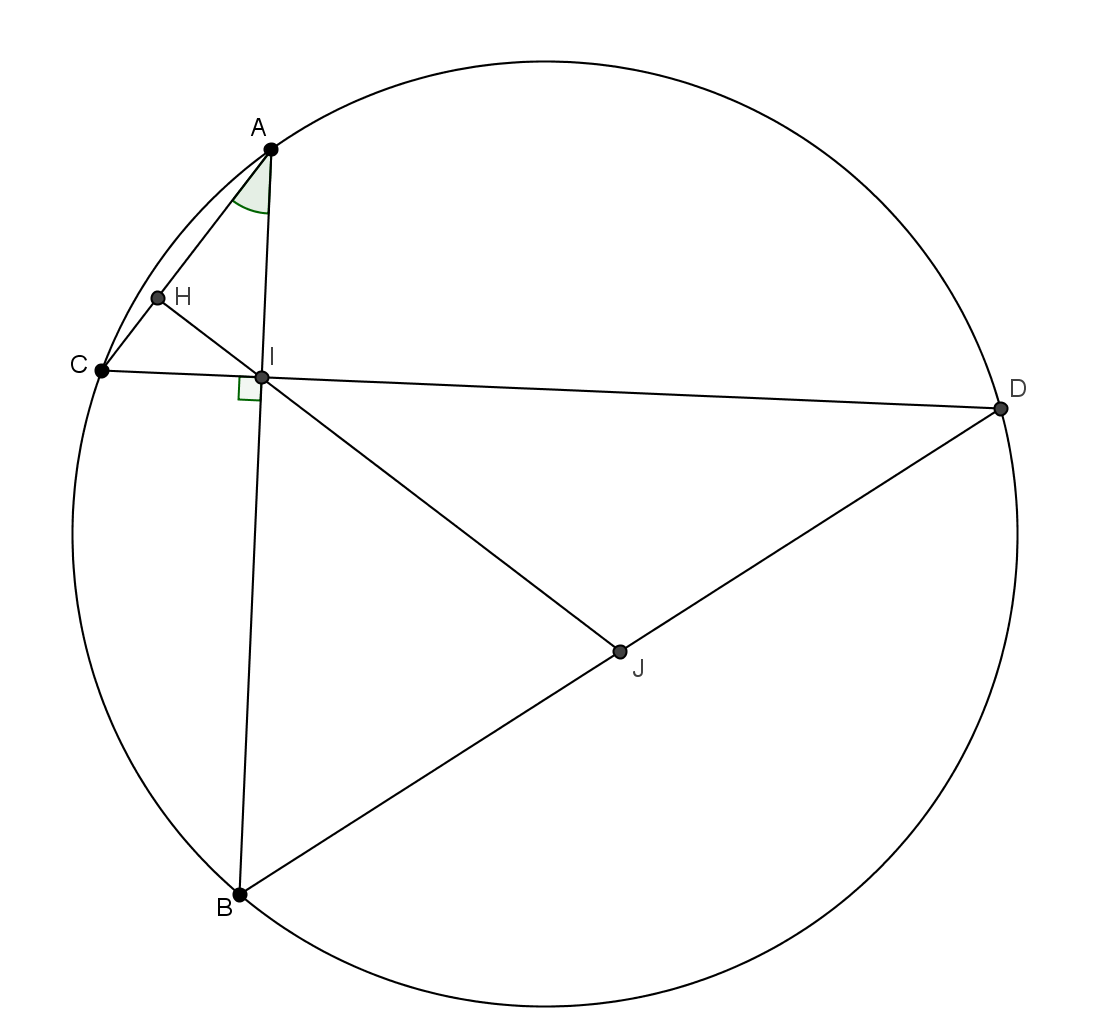
\includegraphics[width=10cm]{image/geogebra.png}
\end{center}
\end{figure}

Sur la figure ci-contre, $A,B,C,D$ sont quatre points d'un cercle tels que les
droites $(AB)$ et $(CD)$ soient perpendiculaire.On note $I$ le point
d'intersection. Le point $J$ est le milieu du segment $[BD]$ et la droite $(IJ)$
coupe le segment $[AC]$ en $H$.

\begin{enumerate}
  \item L'angle $\widehat{IAC}$ mesure $35�$. Faire la figure sur
  \textbf{Geogebra} et l'enregistrer dans le \textbf{dossier ressource} de la
  classe avec le titre : "Nom-pr�nom-DM3-ex1"
  \item Evaluer tout les angles de la figure.
\end{enumerate}
\end{document}
